\documentclass[a4paper]{article}
\usepackage[pdftex]{graphicx}
\usepackage[utf8]{inputenc}
\usepackage{enumerate}
\usepackage{siunitx}
\sisetup{locale=DE} 
\usepackage{icomma}
\usepackage{amssymb}
\usepackage{tikz}
\usepackage{href-ul}
\hypersetup{
	colorlinks=true,
	linkcolor=blue,
	urlcolor=blue}
\usepackage{geometry}
\geometry{a4paper, top=15mm, left=15mm, right=15mm, bottom=15mm,
	headsep=10mm, footskip=12mm}

\begin{document}
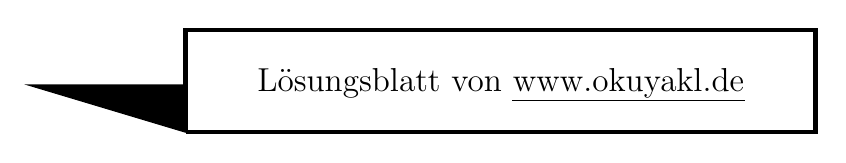
\begin{tikzpicture}(10,3)
	\draw[ultra thick](2,0) --(10,0) -- (10,1.3) --(2,1.3) -- (2,0);
	\draw[fill=black](2,0)-- (0,.6) -- (2,.6) -- (2,0);
	\node at (6,.6) {\large Lösungsblatt von \href{https://www.okuyakl.de}{www.okuyakl.de}};
\end{tikzpicture}
\vspace{0.5 cm}

\noindent{\bf Aufgabe 1. a)}\\
Die Bremsbeschleunigung ist:
$$a= {\Delta v \over \Delta t} ={{108 \over 3,6}~\SI{}{\meter\over \second}\over \SI{0,04}{\second}}=\SI{750}{\meter\over {\second^2}} $$
\vspace{0.5 cm}

\noindent{\bf Aufgabe 1. b)}\\
Die Bremskraft wäre dann:
$$ F = m \cdot a = \SI{0,42}{\kilogram} \cdot \SI{750}{\meter\over {\second^2}}=\SI{315}{\newton}$$
\vspace{0.5 cm}

\noindent{\bf Aufgabe 2. a)}\\
\begin{itemize}
	\item Phase 1: Der Körper bewegt sich mit konstanter Geschwindigkeit.
	\item Phase 2: Er wird bis zum Stillstand abgebremst. 
	\item Phase 3: Beschleunigung 
	\item Phase 4: gleichförmige Bewegung
	\item Phase 5: Abbremsen bis zum Stillstand
\end{itemize}
\vspace{0.5 cm}

\noindent{\bf Aufgabe 2. b)}\\
Der Weg ist die Fläche unter der Kurve. Ein Quadrat entspricht $4~FE=\SI{4}{\meter}$ Wir zählen unter dem Teilstück in Phase 1 8~m, unter dem von Phase 2 4~m.
\vspace{0.5 cm}

\noindent{\bf Aufgabe 2. c)}\\
Insgesamt sind unter den Linien 12,5 Quadrate, also 50~m.
Die Durchschnittsgeschwindigkeit ist:
$$\bar v={\SI{50}{\meter} \over \SI{12}{\second}}=\SI{4,2}{\meter\over \second}$$
\vspace{0.5 cm}

\noindent{\bf Aufgabe 2. d)}\\
Kräfte treten nur in den Beschleunigungs- und Bremsphasen auf:
\begin{itemize}
	\item Phase 2: $$ F = m \cdot {\Delta v \over \Delta t} = \SI{0,75}{\kilogram} \cdot {\SI{-4,0}{\meter\over \second} \over \SI{2}{\second}}=\SI{-1,5}{\newton}$$
	\item Phase 3: $$ F = \SI{0,75}{\kilogram} \cdot {\SI{6,0}{\meter\over \second} \over \SI{2}{\second}}=\SI{2,3}{\newton}$$
	\item Phase 5: $$ F = \SI{0,75}{\kilogram} \cdot {\SI{-6,0}{\meter\over \second} \over \SI{4}{\second}}=\SI{-1,1}{\newton}$$
\end{itemize}
Betragsmäßig ist die Kraft in Phase 3 am größten.
\vspace{0.5 cm}

\noindent
\begin{minipage}{0.6\textwidth}
	\noindent{\bf Aufgabe 2. e)}\\
	Die Formel für die Beziehung zwischen Wegstrecke und Beschleunigung ist:
	$$
	\renewcommand{\arraystretch}{2}
	\begin{array}{rcll}
	v^2 &=& 2 \cdot a \cdot s & |\sqrt{\quad}\\
	v &=& \sqrt{ 2 \cdot a \cdot s}\\
	v &=& \sqrt{{2\cdot \SI{4,0}{\meter\over {\second^2}}}\cdot \SI{32}{\meter}}&=\SI{16}{\meter\over \second}
	\end{array}
	$$
	Die Beschleunigungszeit ist hierbei:
	$$ t = {v \over a} = {\SI{16}{\meter\over \second} \over \SI{4,0}{\meter\over {\second^2}}}= \SI{4,0}{\second}$$
	Der Körper hat nun noch 18~m zurückzulegen; hierfür benötigt er:
	$$ t = {s \over v} = {\SI{18}{\meter} \over \SI{16}{\meter\over \second}}=\SI{1,1}{\second}$$
	Insgesamt braucht er also 5,1~s.
\end{minipage}
\hfill
\begin{minipage}{0.4\textwidth}
\setlength{\unitlength}{1 cm}
\begin{picture}(6,4)
\put(0.5,0.5){\vector(1,0){5.5}}
\put(0.5,0.5){\vector(0,1){4}}
\put(0.5,0){0}
\put(4.2,0.7){Zeit in s}
\put(0.7,3.5){v in $\SI{}{\meter\over \second}$}
\put(0.5,0.5){\line(1,1){2.5}}
\put(3,3){\line(1,0){1.5}}
\end{picture}
\end{minipage}
\vspace{0.5 cm}

\noindent{\bf Aufgabe 3. a)}\\
$$v = { s \over t} = {\SI{5000}{\meter} \over \SI{150}{\second}}=\SI{33,3}{\meter\over \second}$$
$$v = 33,3 \cdot 3,6 = \SI{120}{\kilo\meter\over \hour}$$
\vspace{0.5 cm}

\noindent{\bf Aufgabe 3. b)}\\
$$ t = {s \over v} = {\SI{5400}{\meter}\over \SI{33,3}{\meter\over \second}}= \SI{162}{\second} =\SI{2}{\minute}~\SI{42}{\second}$$
\vspace{0.5 cm}

\noindent{\bf Aufgabe 3. c)}\\
$$ s = v \cdot t = \SI{125}{\kilo\meter\over \hour} \cdot \SI{1,6}{\hour} = \SI{200}{\kilo\meter}$$
\vspace{0.5 cm}

\noindent{\bf Aufgabe 3. d)}\\
Gleichförmige Bewegung; Bewegung ohne Beschleunigung.
\vspace{0.5 cm}

\noindent {\bf Aufgabe 4. a)}
Die Beschleunigung a beträgt ($v=\SI{55,6}{\meter\over \second}$): 
$$ a = {\Delta v \over \Delta t} = {\SI{55,6}{\meter\over\second} \over \SI{10}{\second}}= \SI{5,6}{\meter\over {\second^2}}$$
\vspace{0.5 cm}

\noindent {\bf Aufgabe 4. b)}
Die benötigte Strecke ist:
$$ s = {1 \over 2}a\cdot t^2={1 \over 2}\cdot\SI{5,6}{\meter\over {\second^2}} \cdot (\SI{10}{\second})^2 = \SI{280}{\meter}$$
\vspace{0.5 cm}

\noindent {\bf Aufgabe 4. (i) und (ii)}
Zeit-Geschwindigkeits-Diagramm:
\vspace{0.5 cm}

\setlength{\unitlength}{1 cm}
\begin{picture}(8,6)
\put(0.5,0.5){\vector(1,0){7}}
\put(0.5,0.5){\vector(0,1){5}}
\put(0.5,0){0}
\put(2.0,0){15}
\put(5.0,0){45}
\put(7,0){65}
\put(7.2,0.7){Zeit in s}
\put(0,3.5){60}
\put(0,5){90}
\put(0.7,5){v in $\SI{}{\meter\over \second}$}
\put(0.5,0.5){\line(1,2){1.5}}
\put(2,0.5){\line(0,1){3}}
\put(2,3.5){\line(1,0){3}}
\put(5,0.5){\line(0,1){3}}
\put(5,3.5){\line(4,3){2}}
\put(7,0.5){\line(0,1){4.5}}
\put(1.5,1.5){$A_1$}
\put(3.5,1.5){$A_2$}
\put(5.5,1.5){$A_3$}
\end{picture}
\vspace{0.5 cm}

\noindent Wir bestimmen die Flächen unter der Kurve (=zurückgelegter Weg). $A_1$ ist ein Dreieck,
$A_2$ ein Rechteck und $A_3$ ist ein Trapez.
$$
\begin{array}{ccc}
A_1 =& 0,5 \cdot \SI{15}{\second}  \cdot \SI{60}{\meter\over \second} &= \SI{450}{\meter}\\
A_2 =& \SI{30}{\second} \cdot \SI{60}{\meter\over \second} &= \SI{1800}{\meter}\\
A_3 =& 0,5 \cdot \SI{20}{\second} \cdot (60+90) \SI{}{\meter\over \second} &=\SI{1500}{\meter}  \\
& \textnormal{insgesamt} \, s=& \SI{3750}{\meter}
\end{array}
$$
\begin{center}
	\includegraphics[width=7 cm]{../../viecher/endcomic.pdf}
	
	Hier geht es zurück zum \href{https://www.okuyakl.de/phys/p10kinL410/aa410.pdf}{Aufgabenblatt}
\end{center}

\end{document}

